\chapter{REVISÃO DA LITERATURA}
\label{cap:revisao}

Este capítulo tem como objetivo apresentar um estudo sobre o estado da arte do sistema proposto bem como as principais ferramentas a serem empregadas no desenvolvimento mesmo.

\section{Trabalhos Correlatos}

Esta seção apresenta o estado da arte relacionada aos veículos inteligentes e aplicações, tratando de tópicos relacionados às normas internacionais que regem o ramo. Outro ponto considerado é a definição de tecnologias assistivas ao condutor (ADAS) e também um estudo bibliográfico sobre as técnicas e abordagens relacionadas à modelagem e identificação de comportamento de condutores. 

\subsection{Veículos Inteligentes e Automação Veicular}

A revolução tecnológica que diversos setores têm experimentado se aplica também ao ramo automobilístico. Desde que o primeiro veículo automotor ganhou as ruas no século XIX, tecnologias vem sendo empregadas de forma contínua de tal forma a proporcionar conforto, segurança e economia aos usuários de veículos. Atualmente, a maioria dos veículos em circulação possuem algumas destas tecnologias, como os freios ABS (\textit{Anti-Lock Braking System}) e Programas de Estabilidade Eletrônica (ESP: \textit{Electronic Stability Program}), que de forma contundente proporcionam segurança aos condutores e passageiros por meio do uso de sistemas eletrônicos de alta qualidade.

Esta evolução tecnológica se deve muito à popularização de dispositivos semicondutores que deu início à Era dos Computadores na década de 1970, onde, visto o que o uso de sistemas microprocessados poderiam proporcionar, já se começou a imaginar um futuro onde veículos completamente autônomos estariam inseridos no mercado. 

%A Figura~\ref{fig:aut_car60} apresenta o conceito de veículo autônomo imaginado nos anos de 1960, onde se idealiza um veículo seguidor de linha, sem a necessidade de condutores.

%\begin{figure}[!htb]
%\centering
%\caption{Conceito de carro autônomo na década de 1960.} %legenda
%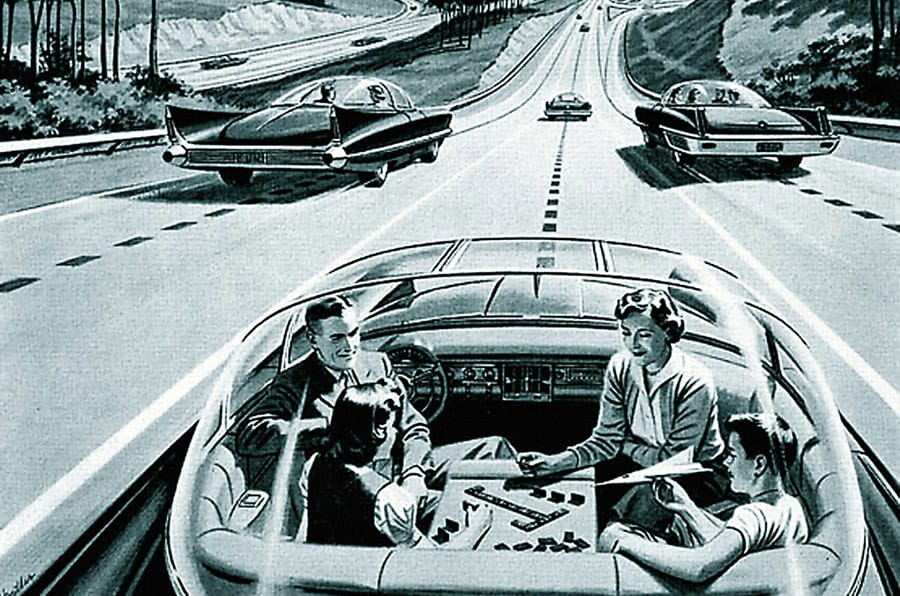
\includegraphics[scale=0.4]{aut_car.jpg}\\  % o 0.9 indica 90% do tamanho original
% pdfLaTeX aceita figuras no formato PNG, JPG ou PDF
% figuras vetoriais podem ser exportadas para eps e depois convertidas para pdf usando epstopdf
%{\small Fonte: Auto-Medienportal.Net/Wikipedia} %Fonte da imagem
%\label{fig:aut_car60} %rotulo para refencia
%\end{figure}

Seguindo a evolução e popularização dos microprocessadores, surgiram assim as Unidades de Controle Eletrônico (ECU). Na indústria automotiva, uma ECU é um dispositivo eletrônico embarcado que realiza a leitura de sinais oriundos de sensores localizados em diversas partes e componentes do veículo e dependendo destas informações colhidas controla várias partes importantes do veículo, como o motor e outras opções automatizadas do veículo \cite{Ebert2009}.

A grande quantidade de informações que passou a circular entre ECU's fez com que surgisse a necessidade de desenvolver uma rede de comunicação multiplexada entre as ECU's, de tal forma a simplificar o cabeamento e reduzir custos de implementação. Assim na década de 80, foi desenvolvido pela Bosch a \textit{Controller Area Network}, ou CAN-bus, que é um barramento intraveicular de comunicação entre ECU's, sensores e atuadores. O CAN-bus é conhecido por sua robustez na transmissão de dados, sendo resistente à interferências eletromagnéticas, e operação em tempo real \cite{Tuohy2014b}. Sendo assim, a crescente capacidade de processamento das ECU's, aliado à grande quantidade de informações relevantes disponíveis no CAN-bus, proporcionaram a introdução do conceito de veículos inteligentes.

Veículos inteligentes, segundo \citeonline{Hubaux2004}, são veículos que são capazes de perceber o ambiente no qual estão inseridos. Um veiculo inteligente deve estar equipado com registradores de dados, processadores, sistemas de posicionamento e geolocalização,  sensores que permitam que o veículo esteja ciente do ambiente, seja no contexto intraveicular, ou no contexto extraveicular. 

No contexto intraveicular, o veículo está ciente de diversos fatores no que diz respeito ao comportamento do condutor, tais como a percepção de fatores neurofisiológicos que podem comprometer a segurança dos usuários, como detecção de sonolência, agressividade ou embriaguez, através de padrões de direção característicos de cada situação. 

No que diz respeito ao contexto extraveicular, o veículo percebe uma série de situações que podem comprometer a segurança dos usuários e, consequentemente, alertar ou até mesmo intervir na dinâmica de direção de modo evitar casualidades. Como exemplos pode-se citar o monitoramento de pontos cegos do veículo, como uma forma de proporcionar ultrapassagens seguras. Sistemas de estacionamento automatizado são outro exemplo deste tipo de sistema, onde o veículo monitora os objetos que o rodeiam e realiza a manobra de estacionamento de forma automática. Outro sistema que visa garantir a segurança dos usuários é o controle de velocidade de cruzeiro, onde o veículo realiza o ajuste da velocidade de acordo com a distância entre o veículo hospedeiro e os veículos à frente. Este sistema é baseado na velocidade do veículo à frente o veículo hospedeiro desacelera ou acelera até a velocidade limiar, tal que a distância entre os veículos seja a estipulada para a segurança dos usuários.

A medida que os veículos inteligentes passam a ser mais sensitivos ao ambiente, mais próximos à total automatização da direção eles estão. Segundo \citeonline{DeWinter2014}, diversos grupos de pesquisa ao redor mundo focam no estudo de veículos autônomos com o objetivo de uma inserção revolucionária do produto no mercado, porém, na prática, este processo é mais evolucionário que revolucionário. Isto se dá pelo fato que ano após ano, novas tecnologias de assistência ao condutor (assunto a ser tratado na próxima seção) são inseridos no mercado, e assim mais automatizada se torna a direção. 


Segundo a norma J3016 da \citeonline{sae2014}, existem seis níveis de automação veicular, desde não automatizado até totalmente automatizado. Dos níveis 0 ao 2 é esperado que o \textit{Condutor Humano} monitore o ambiente de direção e que seja responsável pelas decisões tomadas, porém podem existir sistemas que auxiliem o condutor na tomada de decisões. Por sua vez, nos níveis de 3 a 5, o responsável pelo monitoramento de direção é o \textit{Sistema de Direção Automático}, que pode ser definido como a combinação de diversos sistemas de assistência ao condutor (DAS), porém dos quais não estão inclusos sistemas de intervenção e advertência momentânea pelo fato de não automatizarem partes da tarefa dinâmica de direção e, consequentemente, não mudarem o papel do condutor humano. Os seis níveis de automatização da direção são:

\begin{itemize}
	\item \textbf{SAE Nível 0 - Não Automatizado:} O condutor humano controla todos os aspectos da tarefa dinâmica de condução, mesmo quando auxiliado por sistemas de alerta e intervenção. O condutor humano é responsável pelo monitoramento do ambiente.
	
	\item \textbf{SAE Nível 1 - Assistência ao Condutor:} O modo de direção-execução específica é feito pelo sistema ou pelo condutor, tanto na direção, quanto na aceleração/desaceleração, usando informações do ambiente enquanto o condutor humano é responsável por todas os outros aspectos da dinâmica de condução.
	
	\item \textbf{SAE Nível 2 - Automação Parcial:} O modo de direção-execução específica é feito por um ou mais sistemas de assistência, tanto na direção, quanto na aceleração/desaceleração, usando informações do  ambiente enquanto o condutor humano é responsável por todas os outros aspectos da dinâmica de condução.
	
	\item \textbf{SAE Nível 3 - Automação Condicional:} O modo de direção específica é feito por um sistema automatizado de condução  em todos os aspectos da tarefa dinâmica de condução com a expectativa de que o condutor humano assuma o controle se requisitado.
	
	\item \textbf{SAE Nível 4 - Altamente Automatizado:} O modo de direção específica é feito por um sistema  automatizado de condução em todos os aspectos da tarefa dinâmica de condução, mesmo que o condutor humano não assuma o controle apropriadamente quando requisitado.
	
	\item \textbf{SAE Nível 5 - Totalmente Automatizado:} O modo de direção específica é feito por um sistema  automatizado de condução em todos os aspectos da tarefa dinâmica de condução sob quaisquer condições ambientais.
	
\end{itemize}

Como exemplificação destes níveis de automatização, a Figura~\ref{fig:adas2ad} ilustra os tipos de tecnologias em cada nível SAE, desde somente sistemas avançados de assistência ao condutor, até sistemas de direção automatizados.


\begin{figure}[!htb]
	\centering
	\caption{Exemplos de sistemas de automatização em diferentes níveis.} %legenda
	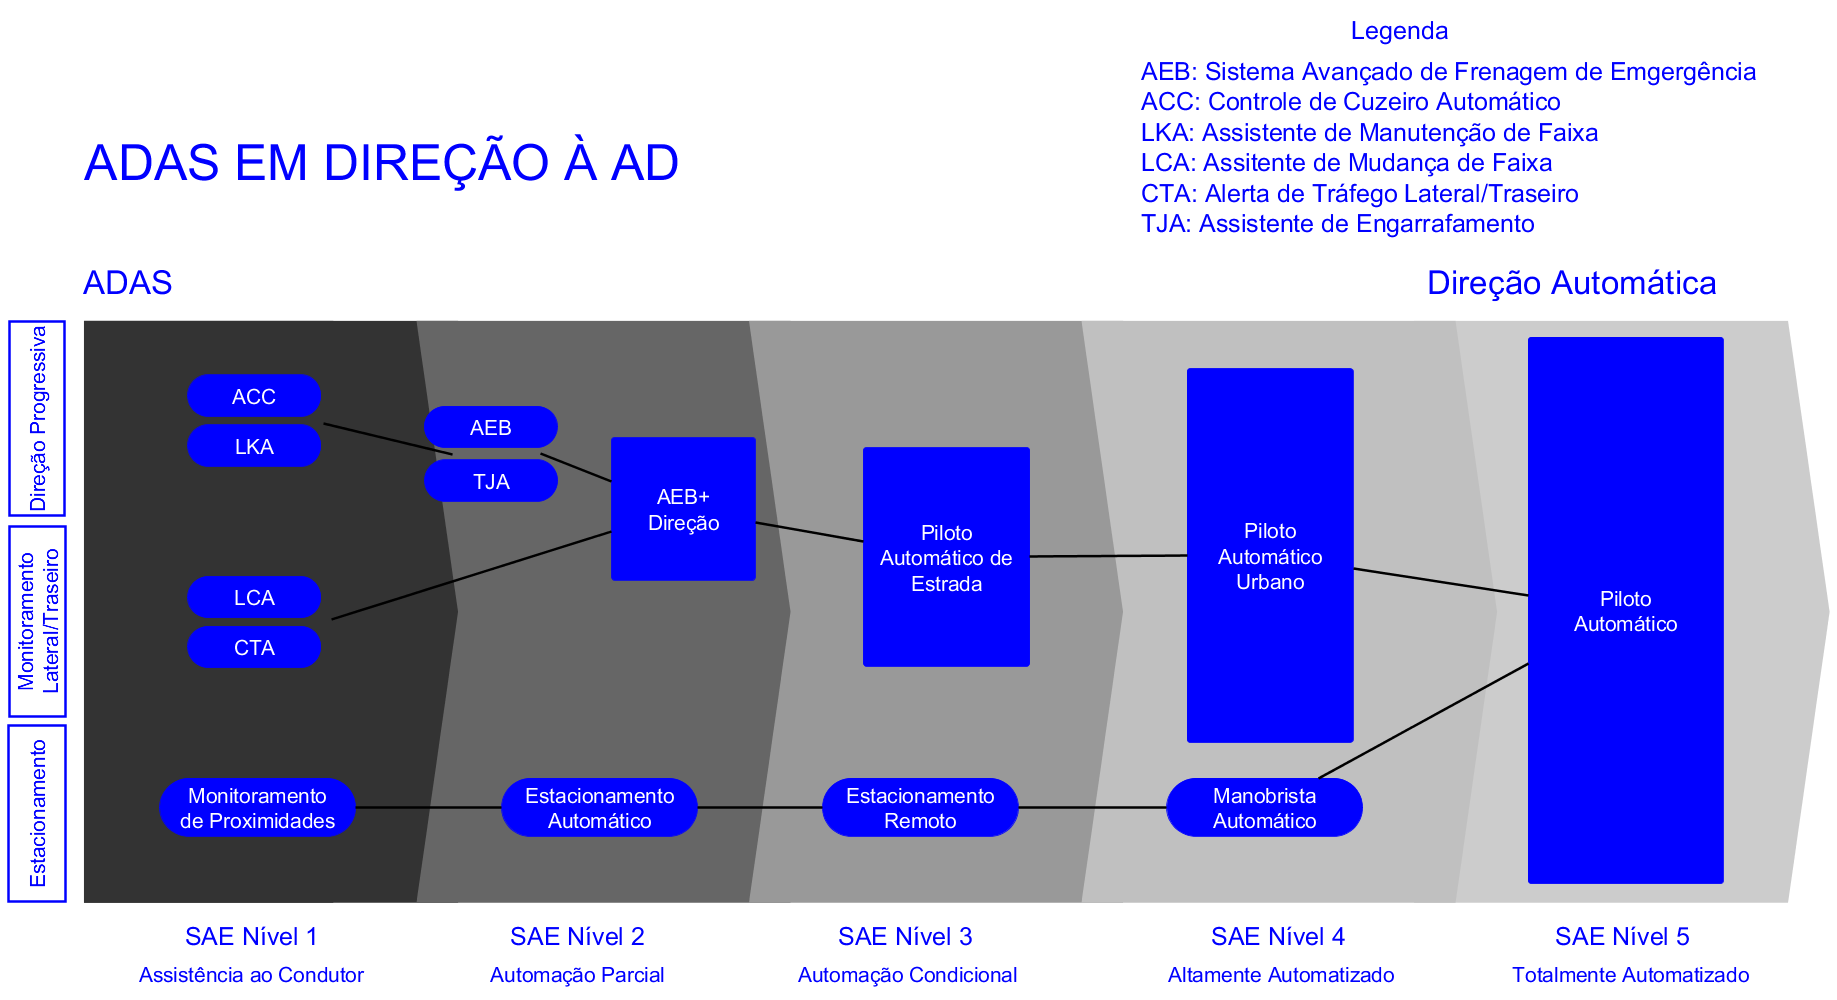
\includegraphics[scale=0.27]{adas2ad.png}\\  % o 0.9 indica 90% do tamanho original
	% pdfLaTeX aceita figuras no formato PNG, JPG ou PDF
	% figuras vetoriais podem ser exportadas para eps e depois convertidas para pdf usando epstopdf
	{\small Fonte: Adaptado de \citeonline{Renesas2017}} %Fonte da imagem
	\label{fig:adas2ad} %rotulo para refencia
\end{figure}



\subsection{Sistemas Avançados de Assistência ao Condutor (ADAS)}

%Desde que o primeiro veículo automotor à combustão interna foi concebido por Carl Benz em 1886, a indústria  automobilística tem experimentado uma constante expansão e penetração em diferentes mercados. Isso se reflete no fato de que a qualidade de vida de uma determinada população é correlacionada com a sua capacidade de mobilidade. Contudo, esta expansão trás à tona uma série de desafios. Além de, obviamente, da redução dos custos financeiros da produção, o consumo de combustível e a implementação e manutenção da infraestrutura (estradas, entre outros) passa por custos de ordem econômico, ambiental e social. Sendo assim a evolução e expansão passa pela redução do consumo de recursos naturais, emissão de gases de efeito estufa e poluição sonora. Somado a isso, fomenta-se a preocupação com congestionamento crescente experimentado por centros urbanos e acidentes de trânsito, umas das principais causa de óbitos e feridos ao redor do mundo.
%
%Hoje, o foco da indústria automotiva pode ser dividido em duas frentes. Em países em desenvolvimento, a indústria tem como foco a redução de custos da produção de tal modo que a oferta de seus produtos se estenda para a população com menor poder aquisitivo. No Brasil, por exemplo, fabricantes têm apostado em carros compactos com baixo consumo de combustível e custo de produção reduzido. Como o pioneiro em sua categoria o Volkswagen Up!, introduzido em 2011, seguido pelo Fiat Mobi (2016) e o Renault Kwid (2017). Porém, tais veículos mencionados são considerados básicos em termos tecnológicos, uma vez que não dispõem de tantos recursos de segurança e conforto aos usuários, com objetivo de justamente oferecer um produto acessível.
%
%Por sua vez, países desenvolvidos, como a Alemanha e Reino Unido, já possuem uma grande penetração de mercado, ou seja, a oferta de veículos à população já está consolidado e quase saturado. Esta situação faz com que as fabricantes de automóveis objetivem a qualidade de seus produtos e a experiência dos usuários. Dentre tais objetivos estão tecnologias que previnam casualidades, reduzam o impacto ambiental e, como consequência, se aumente a eficiência móvel em termos de energia, tempo e recursos.
%
%Um termo frequentemente discutido é a eletrificação dos automóveis que visam reduzir o custo ambiental e conter a crescente escassez de recursos.
%
%
%Contudo, essa expansão trouxe à tona uma série de problemas 

Acidentes de trânsito são uma das maiores causas de mortes na atualidade. A maioria dos acidentes de trânsito são provocados pela desatenção e imprudência dos condutores. Segundo \citeonline{Hoess2009}, 97\% dos acidentes são causados por falha humana. Contudo, grande parte dos estudos são voltados para macro-problemas, como o número de veículos nas vias e gerenciamento de tráfego, e não dão atenção suficiente para decisões individuais de condutores e como isso impacta no tráfego \cite{Carmona2015}. 
Portanto, assistência ao condutor em diferentes níveis são ferramentas potenciais para a segurança dos usuários de veículos e pedestres. Ciente disso, os recentes avanços em inteligência computacional e técnicas de percepção têm proporcionado uma série de novas aplicações desenvolvidas com o propósito de prevenir estes tipos de casualidades utilizando o conceito chamado de Sistemas Avançados de Assistência ao Condutor, ou simplesmente ADAS (\textit{Advanced Driver Assistace System}). 

Segundo \citeonline{Saito2016} os ADAS são baseados em modelos de automação e podem ser categorizados em quatro classes:

\begin{enumerate}
	\item Percepção Aumentada: São todos os sistemas que têm por finalidade monitorar situações em que normalmente o condutor não tem condições de controlar com precisão. Como exemplo estão sensores de estacionamento, monitoramento de ponto cego em mudança de faixa ou ultrapassagem. 
	
	\item Aleta para riscos potenciais: Sistemas que têm intuito de advertir o condutor sobre alguma situação de risco, tais como sonolência/fadiga, pouca distância ao veículo à frente, alerta sobre sobre possíveis falhas nos sistemas do veículo se enquadram nesta classe.
	
	\item Avisos desencadeados: São sistemas que solicitam ao condutor que tome uma ação específica em uma determinada situação de risco. Como exemplos estão alertas de velocidade alta e detecção de sonolência.
	
	\item Controle de segurança automático: Este sistema é acionado quando o condutor não toma providências quando alertado ou a ação de controle do condutor é insuficiente para tal situação de risco.
	
\end{enumerate}

As classes 1 e 2 são implementadas para auxiliar o condutor a perceber ou entender o contexto. Este entendimento determina quais ações devem ser tomadas. Uma vez que decisão de diagnóstico de situação é feita, a seleção de ações efetuadas pelo condutor geralmente é a adequada. Contudo, a decisão tomada pelo condutor pode não ser a correta. Assim a classe 3 auxilia o condutor em tal circunstância. Qualquer ADAS que utilize as classes 1, 2 e 3 são compatíveis com o princípio de automação centrada no ser humano, onde o condutor é a autoridade final no processo de automação. Se o ADAS conter a classe 4, a autoridade passa a ser dividida entre o sistema e o humano. Existem controvérsias sobre o uso da classe 4, uma vez que máquinas altamente automatizadas podem trazer efeitos negativos, como falhas em sensores, erros na malha de controle, complacência, excesso de confiança no sistema, entre outros \cite{Inagaki2012}.


%\section{Modelagem e Identificação de Comportamento do Condutor}

\subsection{Modelagem e Identificação de Comportamento do Condutor}

A revisão bibliográfica feita por \citeonline{Meiring2015} aborda quais algoritmos de inteligência artificial são mais adequados para análise de estilos de direção e comportamento de condutores. É abordado quais os tipos de direção, bem como as causas e consequências de cada um deles (normal/seguro, agressivo, desatento (fadiga, distração), alcoolizado), e aponta o potencial de tais algoritmos em detectar tais condições e prevenir casualidades proporcionadas pelas mesmas. É também realizada uma classificação de técnicas de inteligência computacional e suas aplicações mais comuns são apresentadas na Tabela \ref{tecs1}. Técnicas de inteligência computacional e suas aplicações em ADAS. É concluído que os algoritmos mais promissores para criação de aplicações futuras em ADAS são técnicas baseadas em Lógica Fuzzy, implementação de Modelos Ocultos de Markov (HMM) e Máquinas de Vetor de Suporte (SVM).

\begin{table}[!htb]
	\centering
	\caption{Técnicas de inteligência computacional e suas aplicações em veículos inteligentes. }
	\label{tecs1}
	\begin{tabular}{p{55mm}|p{95mm}}
		\hline
		\multicolumn{1}{c|}{\textbf{Técnica}} & \multicolumn{1}{|c}{\textbf{Aplicações}}                                                                                            \\ \hline
		Redes Neurais Artificiais              & Detecção de sonolência e distração, predição do comportamento do volante, visão computacioal.                                       \\ \hline
		Fast Fourier Transform                 & Detecção de sonolência.                                                                                                             \\ \hline
		Clusterização                          & Distinção de estilo de direção e rotulação de condutor.                                                                             \\ \hline
		Clusterização K-means                  & Identificação individual de condutor e monitoramento de condições de rota.                                                          \\ \hline
		Máquina de estados                     & Reconhecimento de manobras.                                                                                                         \\ \hline
		Máquina de estados finitos             & Modelagem de tomadas de decisão do condutor.                                                                                        \\ \hline
		Máquina de estados híbridos            & Veículos Autônomos.                                                                                                                 \\ \hline
		Lógica Fuzzy                           & Detecção de fadiga, identificação de distração, métodos de pontuação e métodos de reconhecimento de estilo de direção.              \\ \hline
		Modelos Ocultos de Markov (HMM)        & Estimação de comportamento do condutor, reconhecimento de manobras, análise de performance de direção e identificação de distração. \\ \hline
		Técnicas Bayesianas                    & Estimação de comportamento do condutor em situações de dados faltantes.                                                             \\ \hline
		Árvores de decisão                     & Estimação de confiança de resultados em fusão de dados para detecção de sonolência.                                                 \\ \hline
		Modelo de misturas de gaussianas       & Identificação de distração, reconhecimento de manobras e monitoramento de condições de rota.                                       \\ \hline
		Dynamic time warping (DTW)             & Classificação de perfil de risco do condutor e assistentes de direção ou alerta de segurança.                                       \\ \hline
		Filtros de Kalman                      & Predição de processos e modelagem de comportamento humano.                                                                          \\ \hline
		Máquinas de vetor de suporte (SVM)     & Métodos de reconhecimento de estilo de direção, detecção de sonolência e estimação de estado do veículo.                            \\ \hline
		Algoritmos Genéticos                   & Calibração de processos de modelagem de carros adjacentes.                                                                          \\ \hline
	\end{tabular}
	\centering {\small Fonte: Adaptado de \citeonline{Meiring2015}.} %Fonte do quadro
\end{table}

Em seu trabalho, \citeonline{Kumtepe2016} propõem um modelo que faz a fusão de dados provenientes de sensores disponíveis no carro e através de câmeras com o objetivo de se decidir se o condutor apresenta sinais de agressividade ou desatenção. Estas informações são usadas para formar o vetor de características que representam o comportamento do condutor e então são submetidos a uma máquina de vetores de suporte (SVM) de modo a se classificar o condutor testado. O método proposto obteve uma taxa de detecção de agressividade por parte do condutor de 93.1\%.

Por sua vez, \citeonline{Blaszczyk2014} realiza experimentos controlados, onde dois condutores são submetidos a um teste em circuito fechado e dados são coletados por meio da interface OBD-II e Raspberry Pi, além do uso de sensores embarcados em um \textit{smartphone}, com o objetivo de diferencia-los. Utilizando quatro técnicas de classificação (Processo Gaussiano, M5P, \textit{M5Rules} e Tabela de Decisões). O erro médio quadrático (RMSE) para Processo Gaussiano, M5P, \textit{M5Rules} e Tabela de Decisões, foi, respectivamente 0.168, 0.087, 0.023 e 0. Apesar de o erro relativamente baixo, é importante ressaltar que somente dois condutores foram comparados, necessitando assim de mais testes de modo a comprovar a eficácia do sistema.

Seguindo outra vertente, \citeonline{Castignani2015} faz uso somente de \textit{smartphones} para monitorar o comportamento do condutor e alertar para possíveis situações de risco. O uso do dispositivo se justifica pela sua atual penetração no mercado e a facilidade de desenvolvimento de aplicativos, além da robustez dos sensores embarcados nos aparelhos. Um sistema fuzzy é usado para computar o escore de diferentes condutores usando informações em tempo real, como acelerômetros e sistema de navegação GPS provenientes do \textit{smartphone}, aceleração, frenagens e posição do volante, provenientes do barramento CAN do veículo por meio da interface OBD-II, além de topologia da rota e condições climáticas. A validação do sistema é feita através de teste em circuito fechado com diversos condutores.

Técnicas de inteligência computacional híbridas também são exploradas, como no trabalho de \citeonline{Echanobe2016}, onde uma Rede Neural Artificial (RNA) é otimizado por Algorítimos Genéticos Multiobjetivos com a finalidade de realizar a classificação de condutores através de diversos parâmetros de entrada. Testes foram conduzidos com diferentes parâmetros e número de neurônios e camadas, de modo a diminuir o erro da RNA. O resultado obtido é um classificador com menor número de variáveis de entrada em diferentes domínios (tempo, frequência e cepstral), menor quantidade de neurônios e camadas escondidas da RNA e por consequência um sistema mais rápido eficiente no que diz respeito ao custo computacional.

%Contudo, \citeonline{Piotr2015} afirma que a modelagem de comportamento de condutor ainda não são confiáveis o suficiente para aplicação em larga escala, justificando que grande parte dos trabalhos na área foram feitos com experimentos limitados pela quantidade de condutores testados e que somente os sensores utilizados não são suficientes para tal modelagem. Isto ocorre uma vez que as decisões tomadas não são repetitivas, tal qual assumindo por diversos trabalhos. Em cenários repetitivos é possível distinguir entre diferentes tipos de comportamentos, porém, quando o mesmo condutor é submetido a cenários diferentes, a correlação entre os dados é reduzida e muitas vezes é comparada com outro condutor. 

\section{Extração de Características}

Em aprendizado de máquina, reconhecimento de padrões e processamento de imagem, extração de características começa por um conjunto inicial de dados medidos e retorna valores derivados (características) com a intenção de serem informativas e não redundantes. A aplicação destas técnicas facilitam os subsequentes passos de aprendizagem e generalização levando a uma melhor interpretação dos dados. 

\subsection{Estatísticas de Ordem Superior}

O termo Estatística de Ordem Superior (EOS) refere à funções que usam a terceira potência ou superiores de uma certa amostra, diferentemente de Estatística de Ordem Inferior, que fazem uso de termos constantes, lineares e quadráticos (potências zero, um e dois). EOS pode ser definidos em termos de momentos e cumulantes. enquanto momentos são próprios para descrever sinais determinísticos, cumulantes são adequados para a análise de sinais estocásticos (dados de direção podem ser classificados como estocásticos) \cite{guedes2016non}:. 
Considere $x$ como um processo aleatório, real e discreto com média zero. Então, a segundo, terceiro e quarto cumulante podem ser obtidos, respectivamente por 

Dado um caso unidimensional ($d = 1$), os momentos de uma variável aleatória $X$ podem ser definidos como:

\begin{equation}
\begin{matrix}
m_1 = \left \langle x \right \rangle\\ 
m_2 = \left \langle x^{2} \right \rangle\\ 
\vdots \\ 
m_n = \left \langle x^{n} \right \rangle
\end{matrix}
\end{equation}

Então os cumulantes podem ser escritos em forma de momentos:

\begin{equation}
\begin{matrix}
c_1 = m_1\\ 
c_2 = m_2-{m_1}^2=\sigma^2\\ 
c_3 = m_3-3{m_1}{m_2}+2{m_1}^3\\ 
c_4 = m_4 - 3{m_2}^2-4m_1m_3+12{m_1}^2m_2-6{m_1}^4
\end{matrix}
\end{equation}

Os cumulantes $c_1$, $c_2$, $c_3$ e $c_4$ são a média, a variância, a assimetria e a curtose, respectivamente. Dentre os quais somente a média não é uma EOS. Para um sinal discreto $x[n]$, os cumulantes podem ser obtidos ed forma direta por:

\begin{equation}
C_{2,x}(\tau) = \frac{1}{N}\sum_{n=0}^{N-1}x[n]x[mod(n+\tau,N)],
\label{eq:Dcum2}
\end{equation}

\begin{equation}
C_{3,x}(\tau) = \frac{1}{N}\sum_{n=0}^{N-1}x[n]x^2[mod(n+\tau,N)],
\label{eq:Dcum3}
\end{equation}

\begin{equation} \label{eq:cum4}
\begin{split}
C_{4,x}(\tau) = \frac{1}{N}\sum_{n=0}^{N-1}x[n]x^3[mod(n+\tau,N)]-\\
3\frac{1}{N^2}\sum_{n=0}^{N-1}x[n]x[mod(n-\tau,N)].\sum_{n=0}^{N-1}x^2[n]
\end{split}
\end{equation}

\noindent onde $x \in \Re^N$, $\tau=[0, 1,...,N-1]$ são os atrasos, e $mod$ é o operador módulo, que retorna o resto de uma operação inteira \cite{moreirahos}.

Como descrito em~\citeonline{mendel1991}, EOS pode levar a resultados mais representativos quando aplicadas como ferramenta de extração de características em processos não lineares e não gaussianos. De acordo com~\citeonline{naves2016}, a maior vantagem do uso dos cumulantes como extrator de características em problemas de classificação é sua propriedade de imunidade ao ruido gaussiano.


\section{Seleção de Características e Redução de Dimensionalidade}

Uma ferramenta importante para melhorar a eficiência da tarefa de classificação em termos de custo computacional é a redução de dimensionalidade. Esta ferramenta pode ser definida como o processo de redução do número de variáveis de entrada pela obtenção de um conjunto de variáveis principais. Em outros termos, estas técnicas transformam um conjunto de dados de amplo espaço dimensional em um espaço de menor dimensão.

A técnica mais utilizada para redução de dimensionalidade é a Análise de Componentes Principais, descrita posteriormente neste trabalho. Outra técnica que pode ser explorada para esta tarefa é a Análise de Componentes Independentes, embora esta não seja convencionalmente usada para redução de dimensionalidade, mas para a separação de sinais sobrepostos. Contudo, existem exemplos na literatura que aplicam ICA para redução de dimensionalidade \cite{wang2006independent} \cite{cao2003comparison}.

\subsection{Análise de Componentes Principais}

PCA é um procedimento matemático que usa uma transformação ortogonal para para converter um conjunto de variáveis possivelmente correlatadas em um conjunto de variáveis não correlacionadas chamadas de componentes principais \cite{wold1987principal}. Sejam $x_t$($t=1,\ldots,l$ e $\sum_{t=1}^{l}{x_t}=0$) um conjunto de vetores de entrada de $m$ dimensões ${x_t}=({x_t}(1),{x_t}(2),\ldots,{x_t}(m))^T$, então PCA transforma linearmente $x_t$ em um novo vetor $s_t$ pela seguinte expressão:

\begin{equation}\label{eq:pca1}
{s_t} = {U^T}{x_t},
\end{equation}
onde $U$ im uma matriz ortogonal de  $m \times m$ dimensões no qual a  $i$-ésima coluna $u_i$ é o $i$-ésimo autovetor da matriz de covariância  $C$. Portanto, PCA primeiro soluciona o problema dos autovalores:

\begin{equation}\label{eq:pca2}
{\lambda _i}{u_i} = C{u_i}, \qquad i=1,\ldots,m,
\end{equation}
onde $\lambda _i$ é o $i$-ésimo autovalor de $C$ e ${u_i}$ é seu o autovetor relativo. Então, os componentes de ${s_t}$, baseado no obtido em ${u_i}$, são calculados como a transformação ortogonal de ${x_t}$ por:

\begin{equation}\label{eq:pca3}
{s_t}(i) = {u_i}^T{x_t}, \qquad i=1,\ldots,m.
\end{equation}
Estes novos componente ${s_t}(i)$ são os componentes principais. Tal qual a Equação \ref{eq:pca3} demonstra, o número de componentes principais de $s_t$ pode ser reduzido pelo uso de somente alguns dos primeiros autovetores ordenados na ordem descendente dos autovalores. Assim, pode-se concluir que PCA tem a característica de reduzir a dimensão de um conjunto de dados \cite{cao2003comparison}. 

\subsection{PCA Incremental}

O PCA é uma ferramenta útil para problemas para redução de dimensionalidade, porém possui certa limitações quando utilizados em datasets maiores. Isto se dá porque o processamento do PCA é efeito em lotes, que faz com que todos os dados a serem processados devam ser armazenados na memória do dispositivo utilizado. Isto pode ser um problema para aplicações em \textit{hardware} embarcado que tem limitações quanto a capacidade de memória \cite{scikit-learn}.

Diante deste problema, a técnica de PCA Incremental (IPCA) contorna este problema, utilizando uma forma diferente de processamento  que permite cálculos parciais que praticamente obtém nos mesmo resultado do PCA, porém, realizando o processamento em pequenos lotes \cite{Weng2003}.

A versão incremental do algoritmo funciona da seguinte maneira: assume-se que já de posse do conjunto de autovetores $U = [u_j], j = 1,\ldots, p$ do vetor de entrada $x_i, i = 1,\ldots,n$. os autovalores correspondentes são $\lambda = diag(\Lambda)$ e a média dos valores é $\overline{x}$. A construção dos incrementos requer a atualização destes autovalores e autovetores levando em conta uma nova entrada $x_{n+1}$. Primeiramente é feita atualização da média por meio da seguinte expressão\cite{Artac2002}:

\begin{equation}\label{eq:ipca1}
\overline{x}' = \frac{1}{n+1}(n\overline{x} + x_{n+1})
\end{equation}

A atualização dos autovetores é feito pela adição do novo vetor e a aplicando uma transformação rotacional. Para tal, calcula-se o vetor ortogonal residual $h_{n+1} = (Ua_{n+1} + \overline{x})-x_{n+1}$ e em seguida sua normalização $\hat{h}_{n+1}'$. A nova matriz $U'$ é calculada por:

\begin{equation}\label{eq:ipca1}
U' = [U \hat{h}_{n+1}] R,
\end{equation}
\noindent onde $R$ é a matriz de rotação. Este processo é repetido de acordo com o tamanho de lotes definidos (\textit{batch size}). Isto resulta em um processamento mais eficiente em termos de utilização de memória \cite{NIPS2013_5132}.

\subsection{Análise Componentes Independentes}

Análise Componentes Independentes (ICA) \cite{lee1998independent} é uma técnica que originalmente foi desenvolvida para separação cega de fontes, que recupera sinais mutualmente independentes, mas com fontes desconhecidas a partir de suas misturas lineares sem saber os coeficientes de mistura.

ICA considera que os dados são linearmente combinados por um conjunto de fontes independentes e estes sinais podem ser separados de acordo com sua independência estatística \cite{wang2006independent}. Seja $x_t$ a mistura linear e $s_t$ denota o sinal original, então o objetivo do ICA é estimar $s_t$ por:

\begin{equation}\label{eq:ica1}
{s_t} = {U}{x_t},
\end{equation}

\noindent onde $U$ é a matriz $m \times m$ de separação de misturas. Os componentes retornados por $s_t$ são tão independentes estatisticamente quanto possível.

Existem um amplo número de algoritmos que foram desenvolvidos para executar o ICA. Neste trabalho, considerou-se o FastICA de ponto fixo, proposto por \citeonline{hyvarinen1999fast}. Este algoritmo é considerado um dos melhores e mais usados métodos já desenvolvidos. FastICA faz uso de informações mútuas como critério para estimar $s_t$, ao passo que também é uma medida natural de independência entre variáveis aleatórias. A maximização da negentropia (medida do grau de organização do sistema) corresponde à minimização das informações mútuas entre os componentes. Entretanto, esta negentropia não pode ser feita diretamente uma vez que as densidades de probabilidade dos componentes são desconhecidos. A explanação completa do funcionamento do algoritmo FastICA é encontrada em \cite{koldovsky2006efficient}.

As duas principais diferenças entre o PCA e o ICA são, primeiramente, os componentes retornados pelo ICA são estatisticamente independentes, não simplesmente descorrelacionadas tal qual ocorre nos gerados pelo PCA. A segunda distinção é que a matriz  de separação de misturas do ICA não é ortogonal tal qual a do PCA \cite{cao2003comparison}.

\subsection{Análise de Discriminante de Fisher}

Análise de Discriminante de Fisher (FDA) é uma técnica de redução de dimensionalidade, otimizado em termos da maximização da separação entre classes. Dado um conjunto de dados de $n \times m$ dimensões representado pela matriz $X$ com vetor coluna $x_i$, a matriz de dispersão total é dada por \cite{CHIANG20041389}:

\begin{equation}
S_t=\sum_{i=1}^{n}(x_i - \mu)(x_i - \mu)^T
\end{equation}

\noindent onde $\mu$ é o vetor de médias totais dos elementos correspondentes às colunas de $X$. Considerando $X_j$ como o conjuntos de vetores $x_i$ que pertencem à uma determinada classe $j$, ma matriz de dispersão interna para a classe $j$ é

\begin{equation}
S_t=\sum_{x_i\in X_j}^{n}(x_i - \mu_{j})(x_i - \mu_{j})^T
\end{equation}

\noindent onde $\mu_{j}$ é o vetor de médias para a classe $j$. Considerando $c$ o número de classes dos dados, então

\begin{equation}
S_w=\sum_{i=1}^{c}S_i
\end{equation}

\noindent é a matriz de dispersão entre classes, onde $n_j$ é o número de observações na classe $j$.

O primeiro vetor FDA $w_1$ pode ser determinado como:

\begin{equation}
\underset{w_1}{\textrm{argmax}} \frac{{w_1}^TS_bw_1}{{w_1}^TS_ww_1}
\end{equation}

O segundo vetor FDA é calculado de modo a maximizar a dispersão entre classes enquanto minimiza a dispersão entre classes entre todos os eixos perpendiculares com o primeiro vetor FDA em seguida com os vetores FDA restantes. Pode ser provado matematicamente que os vetores FDA são iguais aos autovetores $w_k$ do problema de autovalores generalizados

\begin{equation}
S_bw_k = \lambda_jS_ww_k,
\end{equation}

\noindent onde os autovalores $\lambda_k$ indicam o grau geral de separabilidade entre as classes pela projeção de todas as classes em $w_k$. Com os vetores FDA calculados, as observações são então classificadas de forma a reduzir o espaço dos vetores FDA através de uma análise discriminante \cite{sugiyama2007dimensionality}.


\section{Algoritmos de Classificação Não-Incrementais (\textit{Batch})}

Em Aprendizado de Máquina, mais especificamente em Aprendizado Supervisionado, classificação é o problema de identificar em qual classe um conjunto de observações pertence, com base em um conjunto de dados de treinamento o qual as classes são conhecidas.  Identificação de condutores se enquadra neste problema, uma vez que o objetivo do sistema a ser desenvolvido pelo presente trabalho é reconhecer se um condutor é ou não autorizado a conduzir o veículo. De tal modo, esta seção tem o objetivo apresentar algumas técnicas de Aprendizado de Máquina para problemas de classificação.


\subsection{K-Nearest Neighbors}

$k$-\textit{Nearest Neighbors} (kNN) é uma das mais simples e fundamentais técnicas de classificação, adequada principalmente para casos onde não se tem conhecimento \textit{a priori} sobre a distribuição dos dados utilizados. De acordo com~\citeonline{peterson2009k}, a classificação kNN foi desenvolvida pela necessidade de realizar análise discriminante quando estimativas paramétricas confiáveis de densidades de probabilidade são desconhecidos ou de difícil determinação. A ideia principal do kNN é determinar a classe de uma amostra, baseado nas amostras vizinhas provenientes de um conjunto de treinamento.

O classificador kNN é predominantemente baseado na distância Euclidiana entre as amostras de teste e a amostra de treino especificada. Considerando que $\textbf{x}_i$ são as amostras de entrada com $p$ atributos $(x_{i1}, x_{i2},\ldots, x_{ip})$, $n$ é a quantidade total de amostras de entrada $(i=1,2,\ldots,n)$ e $p$ a quantidade total de atributos $(j=1,2,\ldots,p)$. A distância Euclidiana $d$ entre as amostras $\textbf{x}_i$ e $\textbf{x}_l (l=1,2,\ldots,n)$ é definida por:

\begin{equation}
	d({\textbf x}_i,{\textbf x}_l) = \sqrt{(x_{i1}-x_{l1})^2 + (x_{i2}-x_{l2})^2 + \cdots + (x_{ip}-x_{lp})^2}
\end{equation}

Esta distância $d$ é utilizada determinar a classe de treinamento que um determinado elemento desconhecido pertença, o classificador kNN realiza a busca por $k$ elementos do conjunto de treinamento que estejam mais próximos deste elemento desconhecido, isto é, elementos com maior proximidade a este. O kNN é um classificador que possui somente um parâmetro de entrada ($k$-vizinhos) que normalmente é um número ímpar, para que se evite empates entre as classes e obtido empiricamente ou com o auxílio de técnicas de otimização.

A Figura~\ref{fig:knn_esquema} ilustra um exemplo simples de classificação utilizando o kNN, onde um elemento desconhecido $x_q$ é inserido no espaço amostral de classes conhecidas. São obtidos os cinco elementos mais próximos à $x_q$ e é determinada a classe deste a partir da classe com mais elementos dentro deste espaço de busca. 

\begin{figure}[!htb]
	\centering
	\caption{Exemplo de classificação kNN com $k = 5$.}
	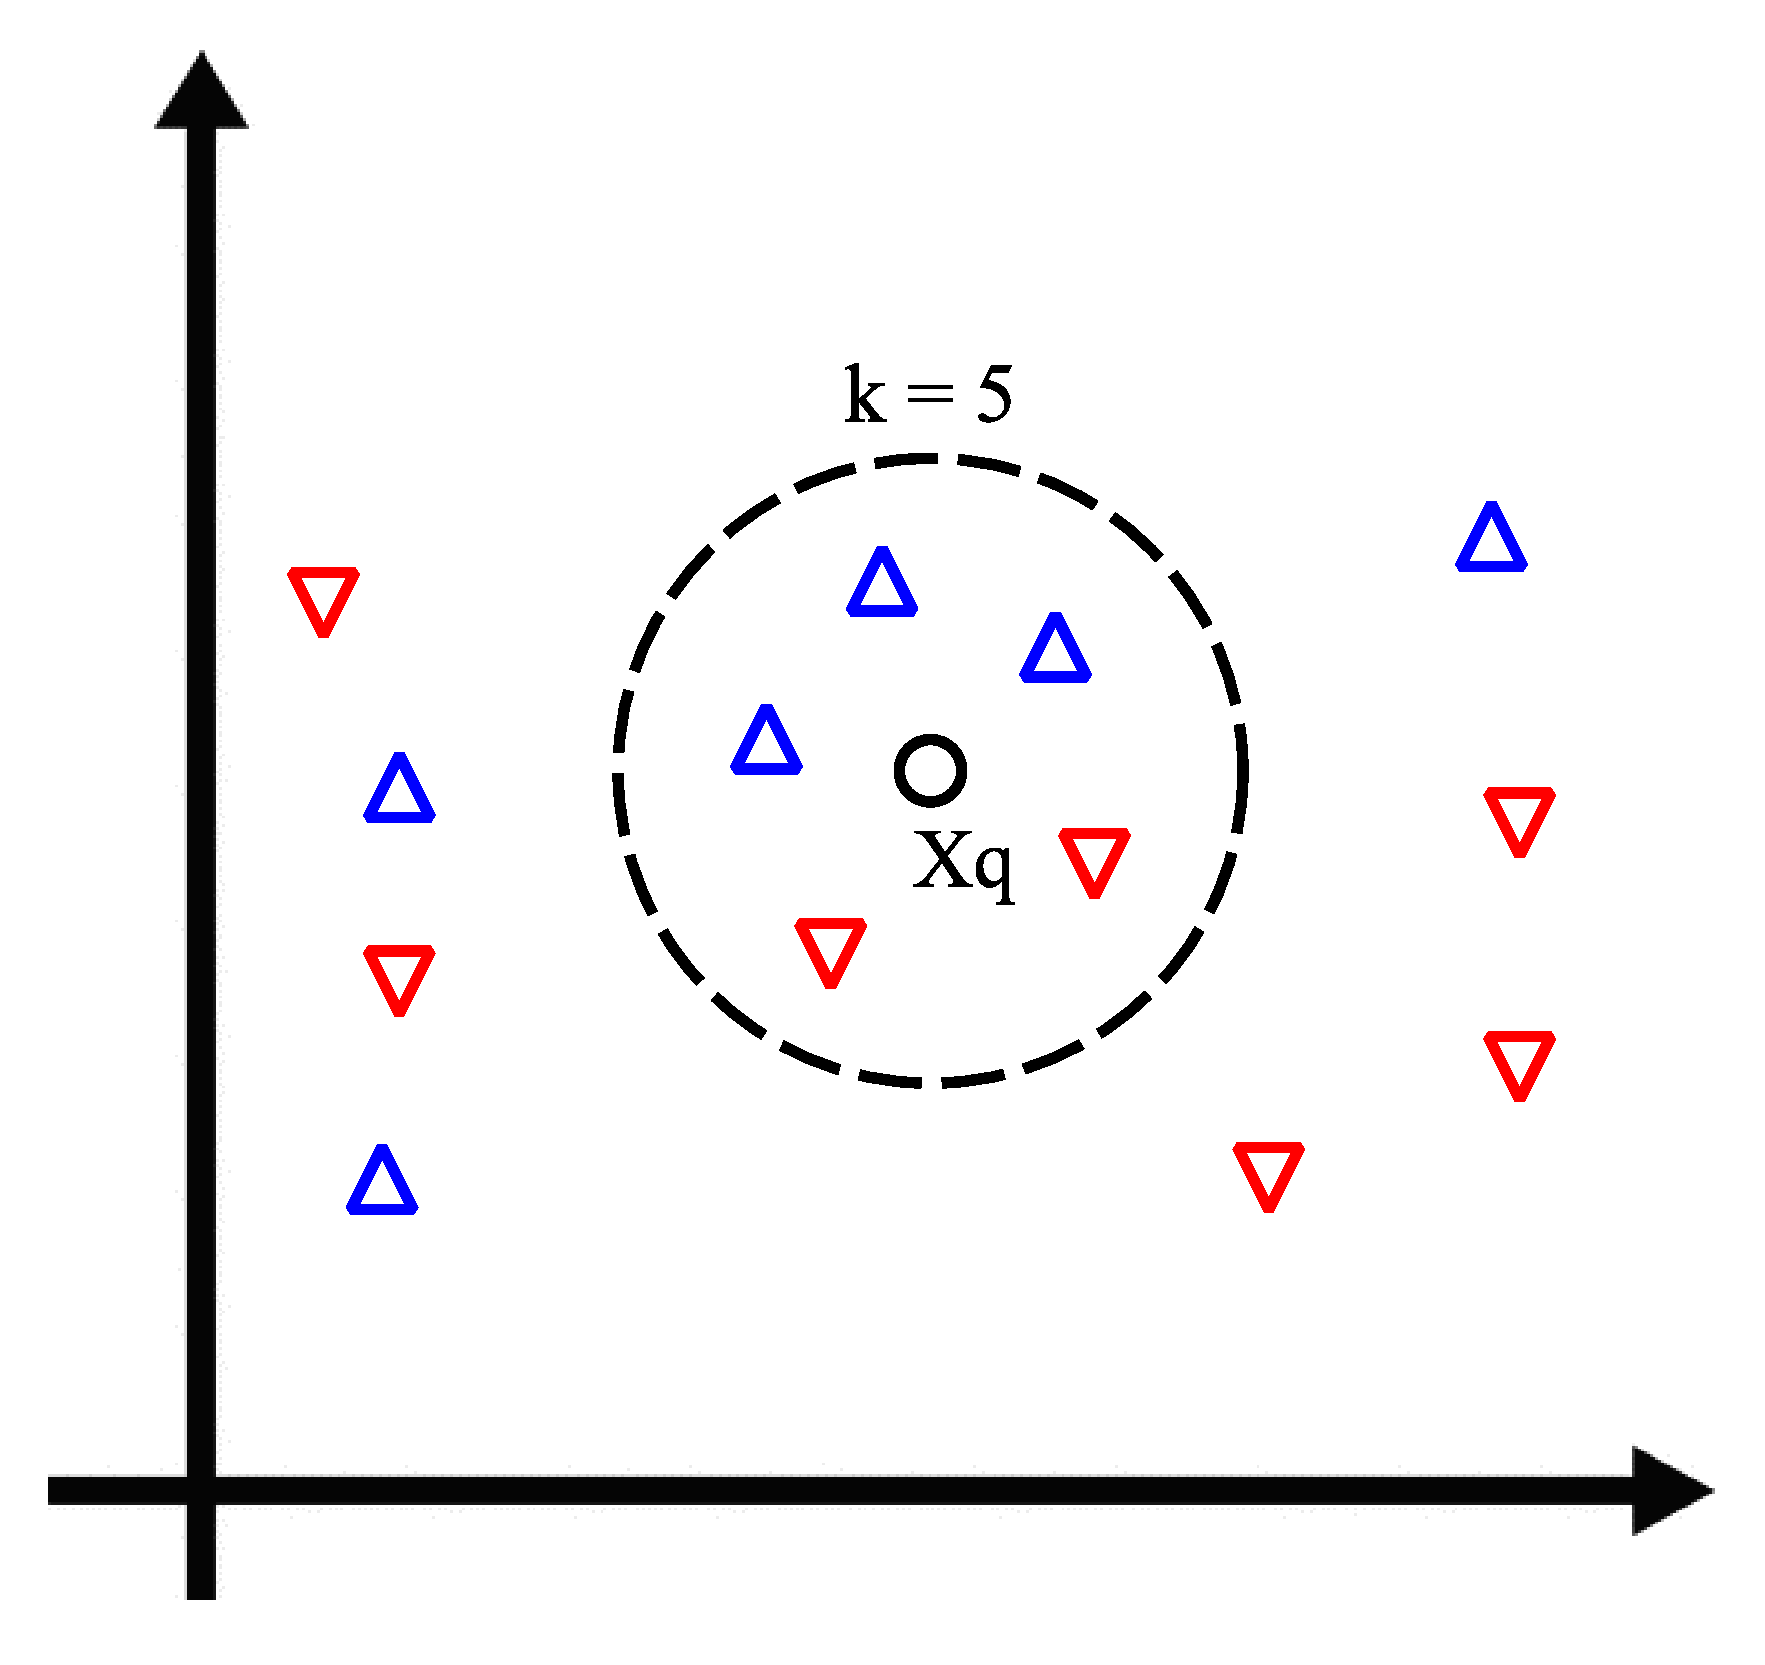
\includegraphics[width=0.6\linewidth]{knn_esquema.eps}\\
	{\small Fonte: Elaborado pelo Autor (2018).}
	\label{fig:knn_esquema}
\end{figure}

\subsection{Florestas Aleatórias}

Florestas Aleatórias (tradução literal de \textit{Randon Forest}) é uma técnica de inteligência computacional para classificação e regressão introduzido por~\citeonline{Breiman2001} que consiste no agrupamento de diversas árvores de decisão~\cite{safavian1991survey} de maneira que sua estrutura seja composta de forma aleatória (ver Figura~\ref{fig:rf_esquema}). Em árvores de decisão comuns, cada nó é dividido de modo a se obter a melhor divisão entre as variáveis do problema em questão. Por sua vez, florestas aleatórias cada nó é dividido usando o melhor entre os subconjuntos de preditores escolhidos aleatoriamente no nó em questão. O classificador requer somente a configuração de dois parâmetros de entrada para a geração do modelo de predição: o número de árvores de decisão desejadas ($n_{tree}$) e o número de variáveis de predição ($m_{try}$) usados em cada nó para o crescimento da árvore.

\begin{figure}[!htb]
	\centering
	\caption{Representação de uma Floresta Aleatória com $n$ Árvores de Decisão.}
	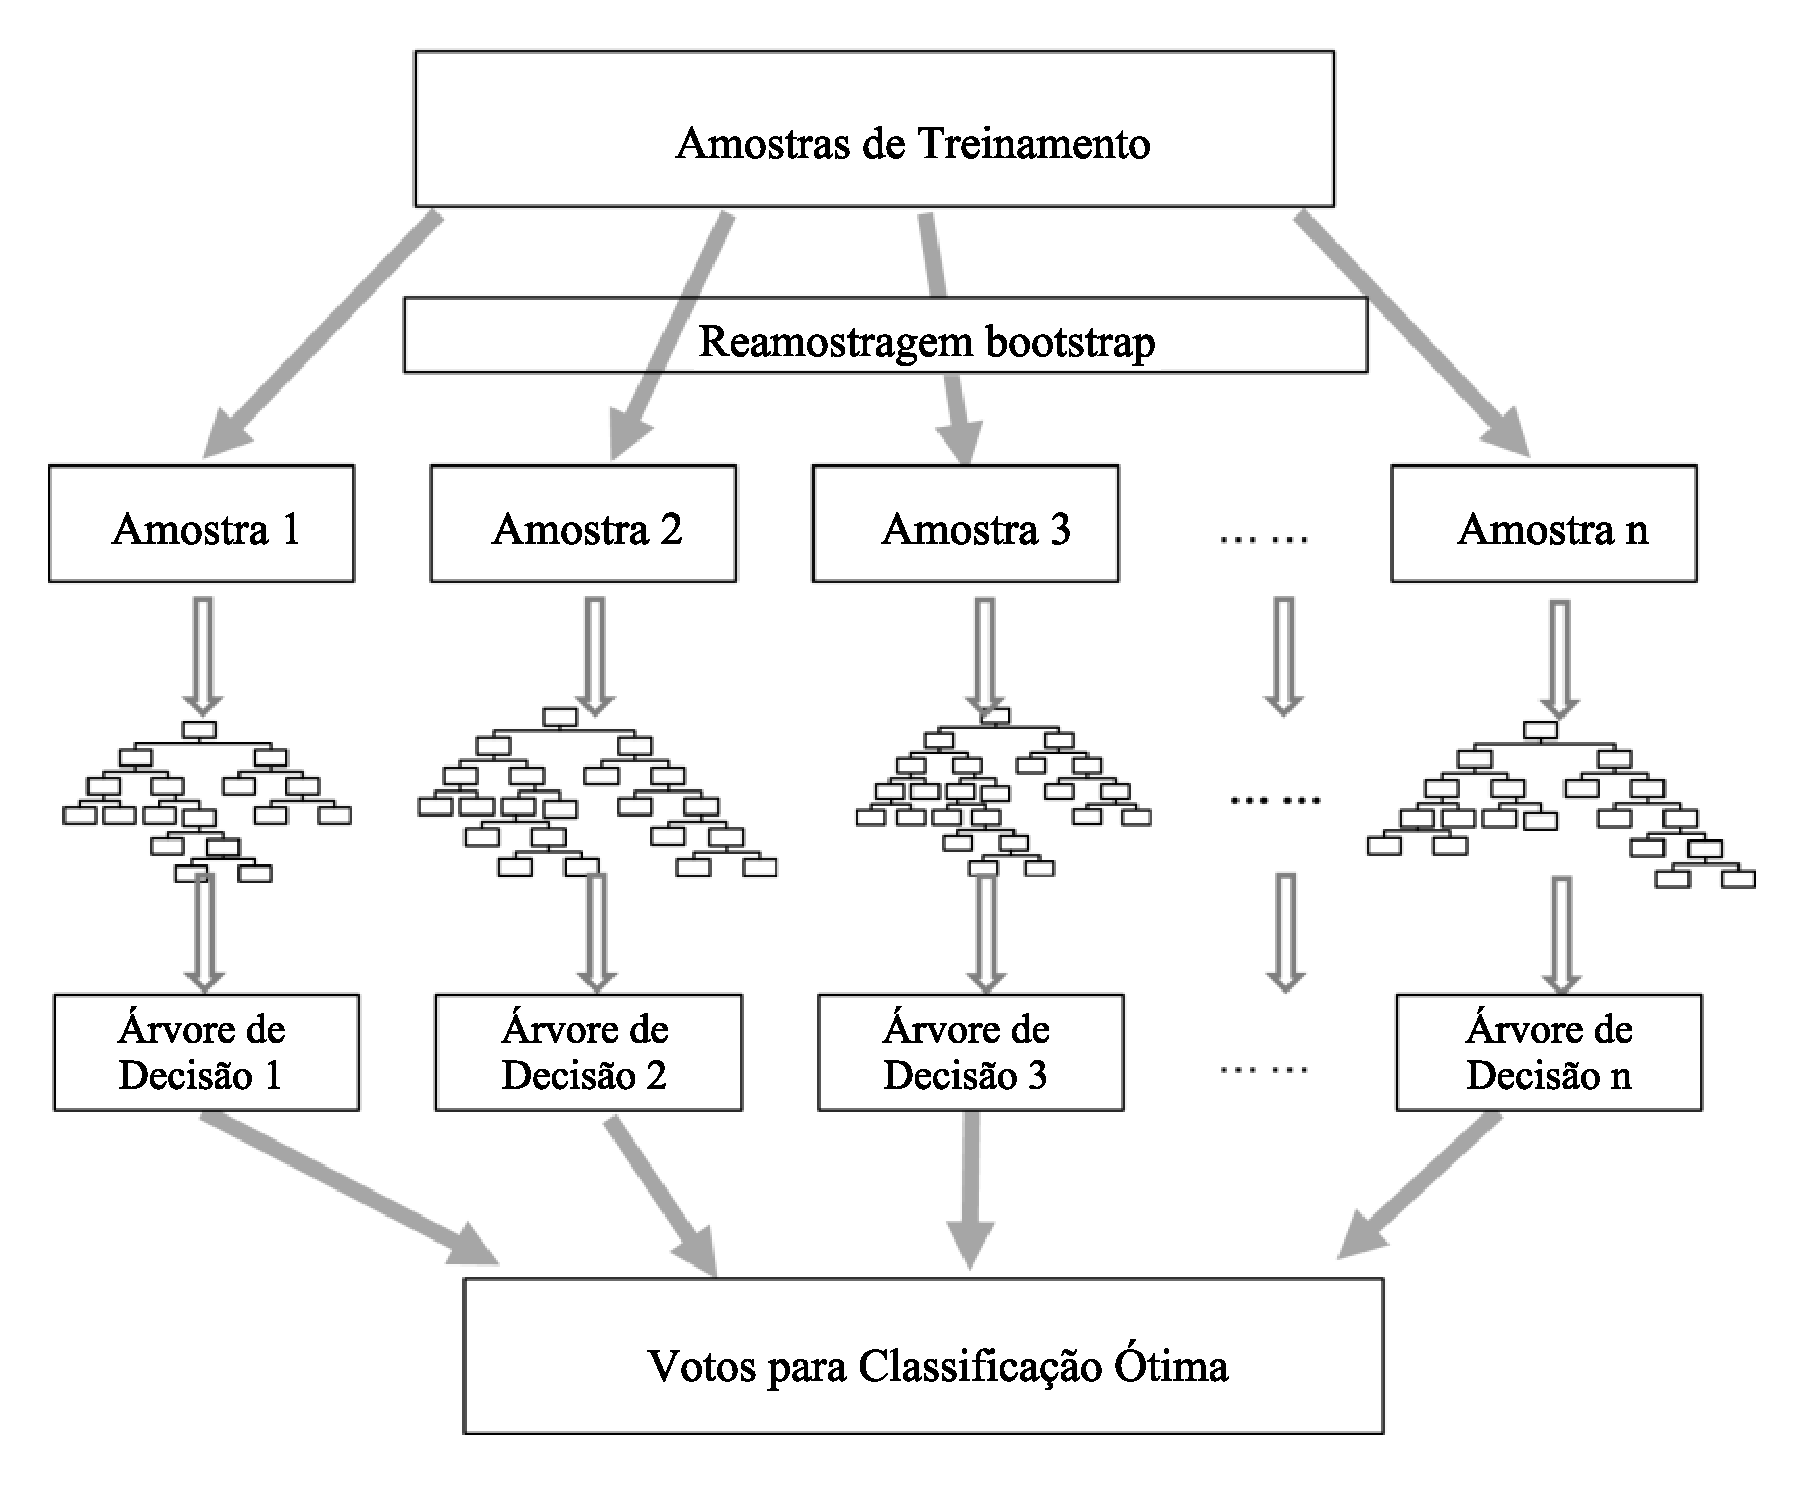
\includegraphics[width=0.8\linewidth]{RF_esquema.eps}\\
	{\small Fonte: Adaptado de \citeonline{zang2017}.}
	\label{fig:rf_esquema}
\end{figure}

Esta estratégia produz resultados satisfatórios se comparados a outros classificadores, incluindo análise discriminante, máquinas de vetor de suporte e redes neurais artificiais, além de ser robusto contra o problema de \textit{overfitting} (ou sobre-ajuste: quando um modelo se ajusta satisfatoriamente ao conjunto de dados treinado, mas se mostra ineficaz para prever novos resultados) \cite{breiman1999random} e boa imunidade à ruido gaussiano~\cite{zang2017}. Porém, apesar desta imunidade com relação ao \textit{overfitting} as florestas aleatórias tendem a saturarão do erro final, isto é, o erro se estagna em um ponto mesmo com a inserção de novas árvores à floresta.
 

\subsection{Redes Neurais Artificiais}

Umas das mais difundidas técnicas de Aprendizado de Máquina, as Redes Neurais Artificiais (RNAs) são amplamente empregadas na solução de diversos problemas de regressão e classificação, atribuindo seu sucesso à sua flexibilidade de síntese de mapeamento multidimensional não-linear de varáveis dependentes e independentes, devido a sua capacidade de aproximação universal.

RNAs são formadas por conjuntos de diversos neurônios artificais, estes propostos por McCulloch e Pitts em 1943. Este modelo de neurônio consiste em receber sinais de entrada $x_n$ nos dentritos do neurônio e retorna um único sinal de saída $y$ no axônio do mesmo. Este modelo é apresentado na Figura~\ref{fig:neuronio-artificial}.

\begin{figure}[!htb]
	\centering
	\caption{Representação de um neurônio artificial não linear.}
	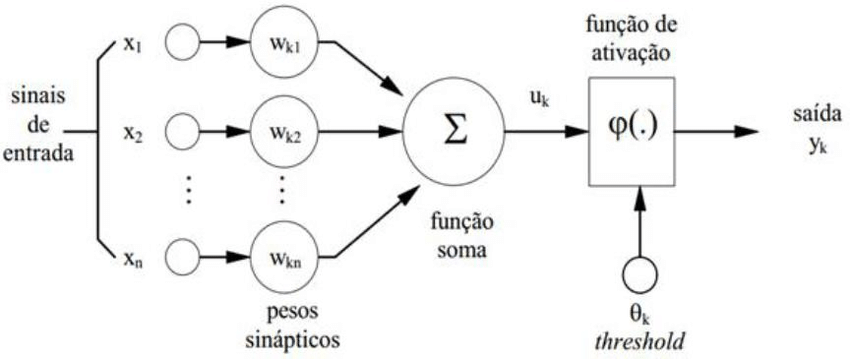
\includegraphics[width=0.6\linewidth]{neuronio-artificial.jpg}\\
	{\small Fonte: Adaptado de \citeonline{haykin2009neural}.}
	\label{fig:neuronio-artificial}
\end{figure}

A expressão que representa este neurônio, com função de ativação unitária, é apresentado pela Equação~\ref{eq:neuronio},

\begin{equation}
	u_k = y_k = \sum _{i=1}^{m}{w}_{i}{x}_{i}+b
	\label{eq:neuronio}
\end{equation}

\noindent onde $x_i$ são as entradas dos neurônios, $w_i$ são os pesos das entradas, $b$ é o \textit{bias} e $y$ é a saída para uma função de ativação unitária. A função de ativação é o elemento que determina  a saída do neurônio em termos do potencial de ativação, muitas das vezes limitando a saída entre $\{0, 1\}$ e $\{-1, 1\}$. Dentre as funções mais utilizadas para esta operação estão as funções sigmoidal, linear, tangente hiperbólica, logarítmica e senoidal.

As combinações destes neurônios formam uma Rede Neural Artificial. Dentre as muitas arquiteturas utilizadas, a mais comum é a rede com múltiplas camadas. \citeonline{haykin2009neural} definu estas redes como sendo um conjunto de unidades sensoriais que constituem a camada de entrada, uma ou mais camadas ocultas e uma camada de saída. Estas redes são conhecidas como Perceptron Multicamadas (\textit{Multilayer Perceptron} - MLP) \cite{rosenblatt1962principles}. Na Figura~\ref{fig:mlp}, é apresentado um modelo de uma MLP com duas camadas escondidas (\textit{hidden layers}).

\begin{figure}[!htb]
	\centering
	\caption{Representação de uma MLP com duas camadas escondidas.}
	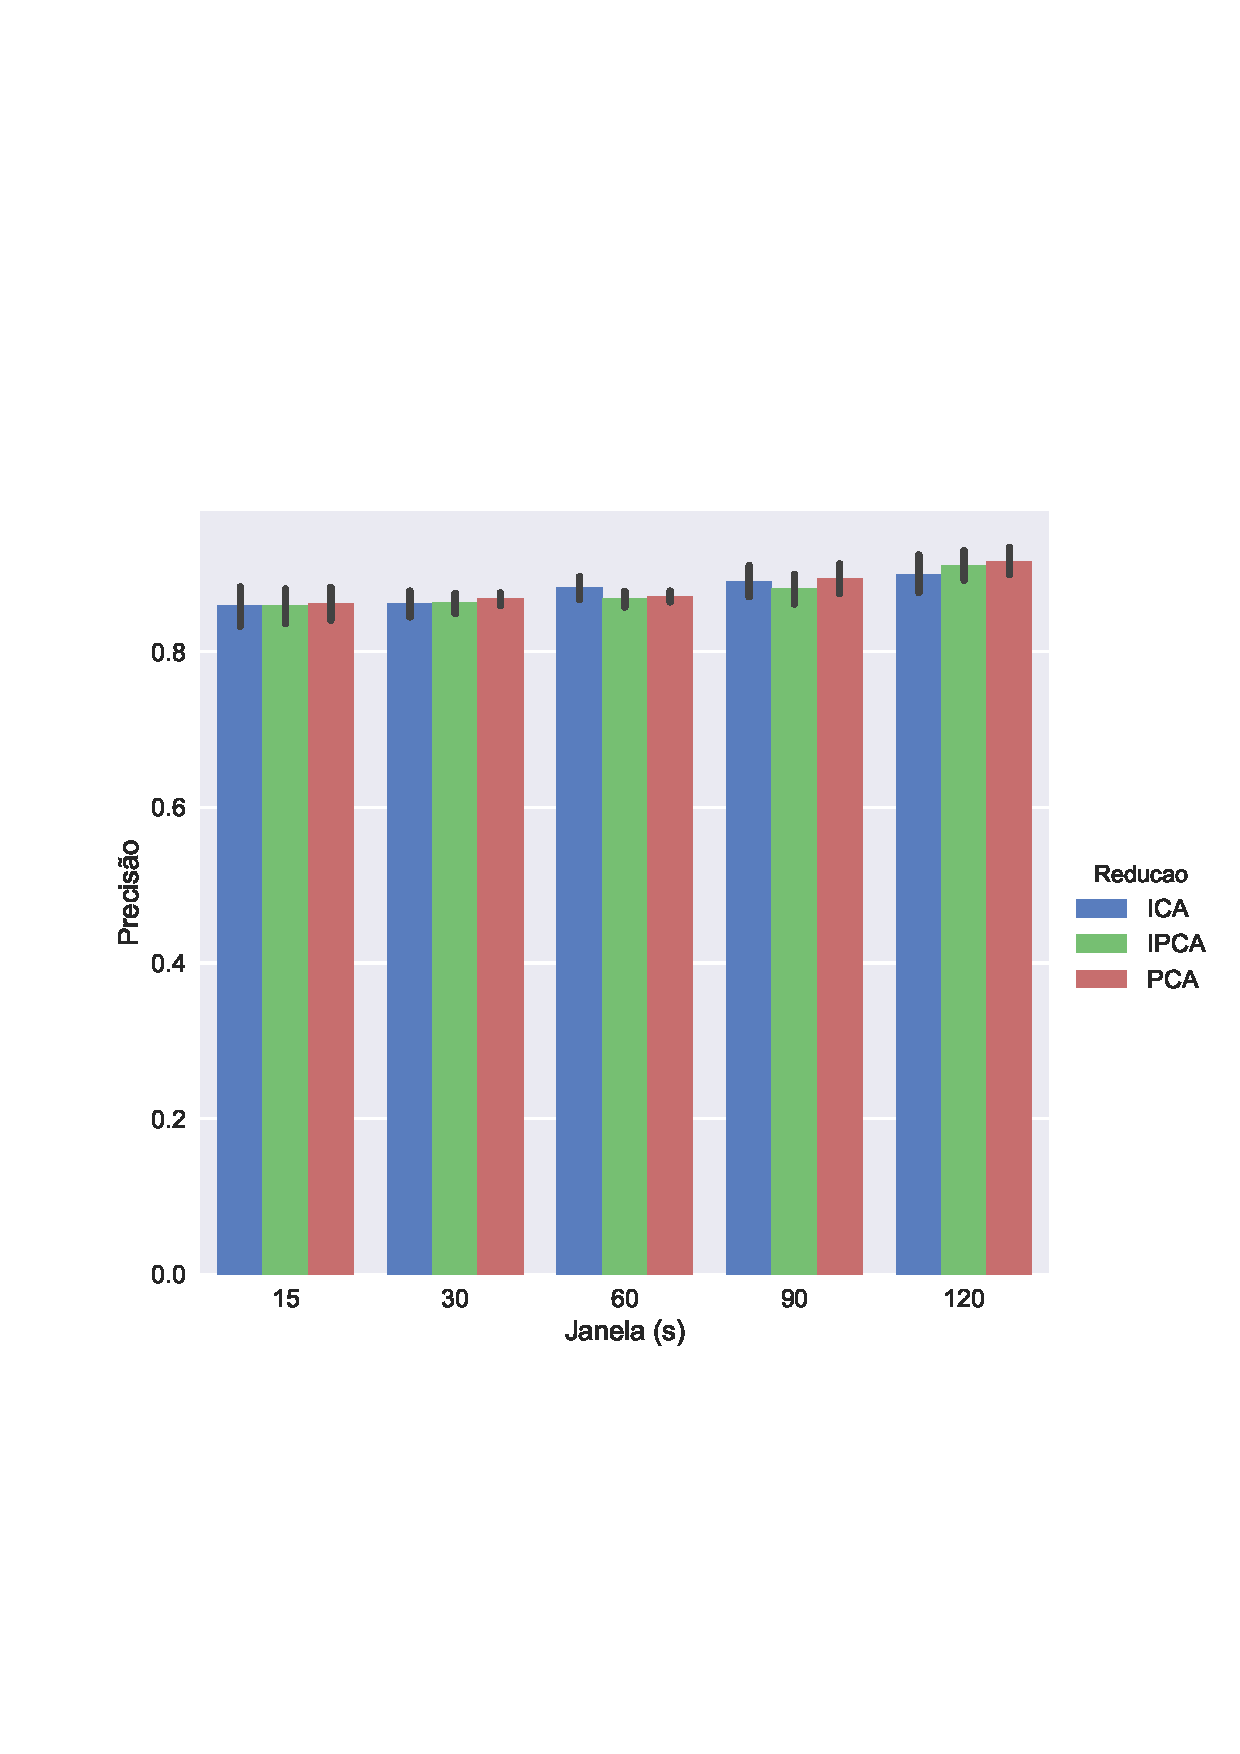
\includegraphics[width=0.8\linewidth]{MLP.png}\\
	{\small Fonte: Adaptado de \citeonline{haykin2009neural}.}
	\label{fig:mlp}
\end{figure}

Existem diveras estratégias de treinamento supervisionado para RNAs, sendo o mais difundido o algoritmo de retro-propagação de erro (\textit{error backpropagation}). Treinamento supervisionado é definido como o estímulo de uma entrada $x$ e a saída da rede $y$ é comparada com o valor desejado (valor real). A partir desta diferença os pesos são ajustados até que o resultado desejado seja obtido. Existem diversas RNAs com arquiteturas diferentes da MLP desenvolvidas, podendo-se destacar as Máquimas de Aprendizado Extremo (\textit{Extreme Learning Machines} - ELM) \cite{huang2006extreme}, Funções de Base Radial (\textit{Radial Basis Function} - RBF) \cite{powell1987algorithms} e Mapas Auto-Organizados (\textit{Self-organizing Maps} - SOM) \cite{VanHulle2012}.

\section{Algoritmos de Classificação Incrementais (\textit{Online})}

Técnicas de aprendizado não-incrementais têm algumas restrições que podem interferir no desempenho do modelo computacional, sendo estas \cite{fontenla2013online}:
\begin{enumerate}
	\item Necessidade de se ter, no momento do treinamento, todo o conjunto de dados para ajuste do modelo preditivo. A cada etapa do processo de aprendizado existe a necessidade do acesso imediato e completo do conjunto de dados.
	
	\item Não pode haver restrições de tempo, isto é, é preciso aguardar o tempo suficiente para o ajuste completo do modelo seja realizado.
	
	\item O processo subjacente aos dados de treinamento não pode sofrer mudanças. Uma vez que o modelo é ajustado, não são necessárias adaptações do mesmo desde que o processo relacionado não sofra mudanças.
\end{enumerate}

Estas restrições supracitadas se aplicam ao problema de identificação de condutores, uma vez que se trata de identificar o modo no qual o condutor opera o veículo. Este processo subjacente pode sofrer mudanças a todo o momento, dependendo de fatores temporais (horário, dia da semana) e climáticos (chuva, nevoeiro), e até mesmo alterações inerentes à estes, como uma mudança de hábitos de direção. Sendo assim, para implementações reais deste sistema, deve-se considerar outro paradigma de aprendizado de máquina para a realização da tarefa de classificação: o Aprendizado Incremental ou \textit{Online}.

Aprendizado de Máquina Incremental é um método dentro de Inteligência Computacional em que os dados tornam-se disponíveis sequencialmente e são usados para a atualização do preditor para aprimora-lo para a predição de dados futuros \cite{fontenla2013online}. A Figura~\ref{fig:apdz} apresenta graficamente a comparação do procedimento de aprendizado dos modelos de predição para algoritmos \textit{Batch} e \textit{Online}.

\begin{figure}[!htb]
	\centering
	\caption{Representação as diferenças de algoritmos de aprendizado Incremental e Não-Incremental.}
	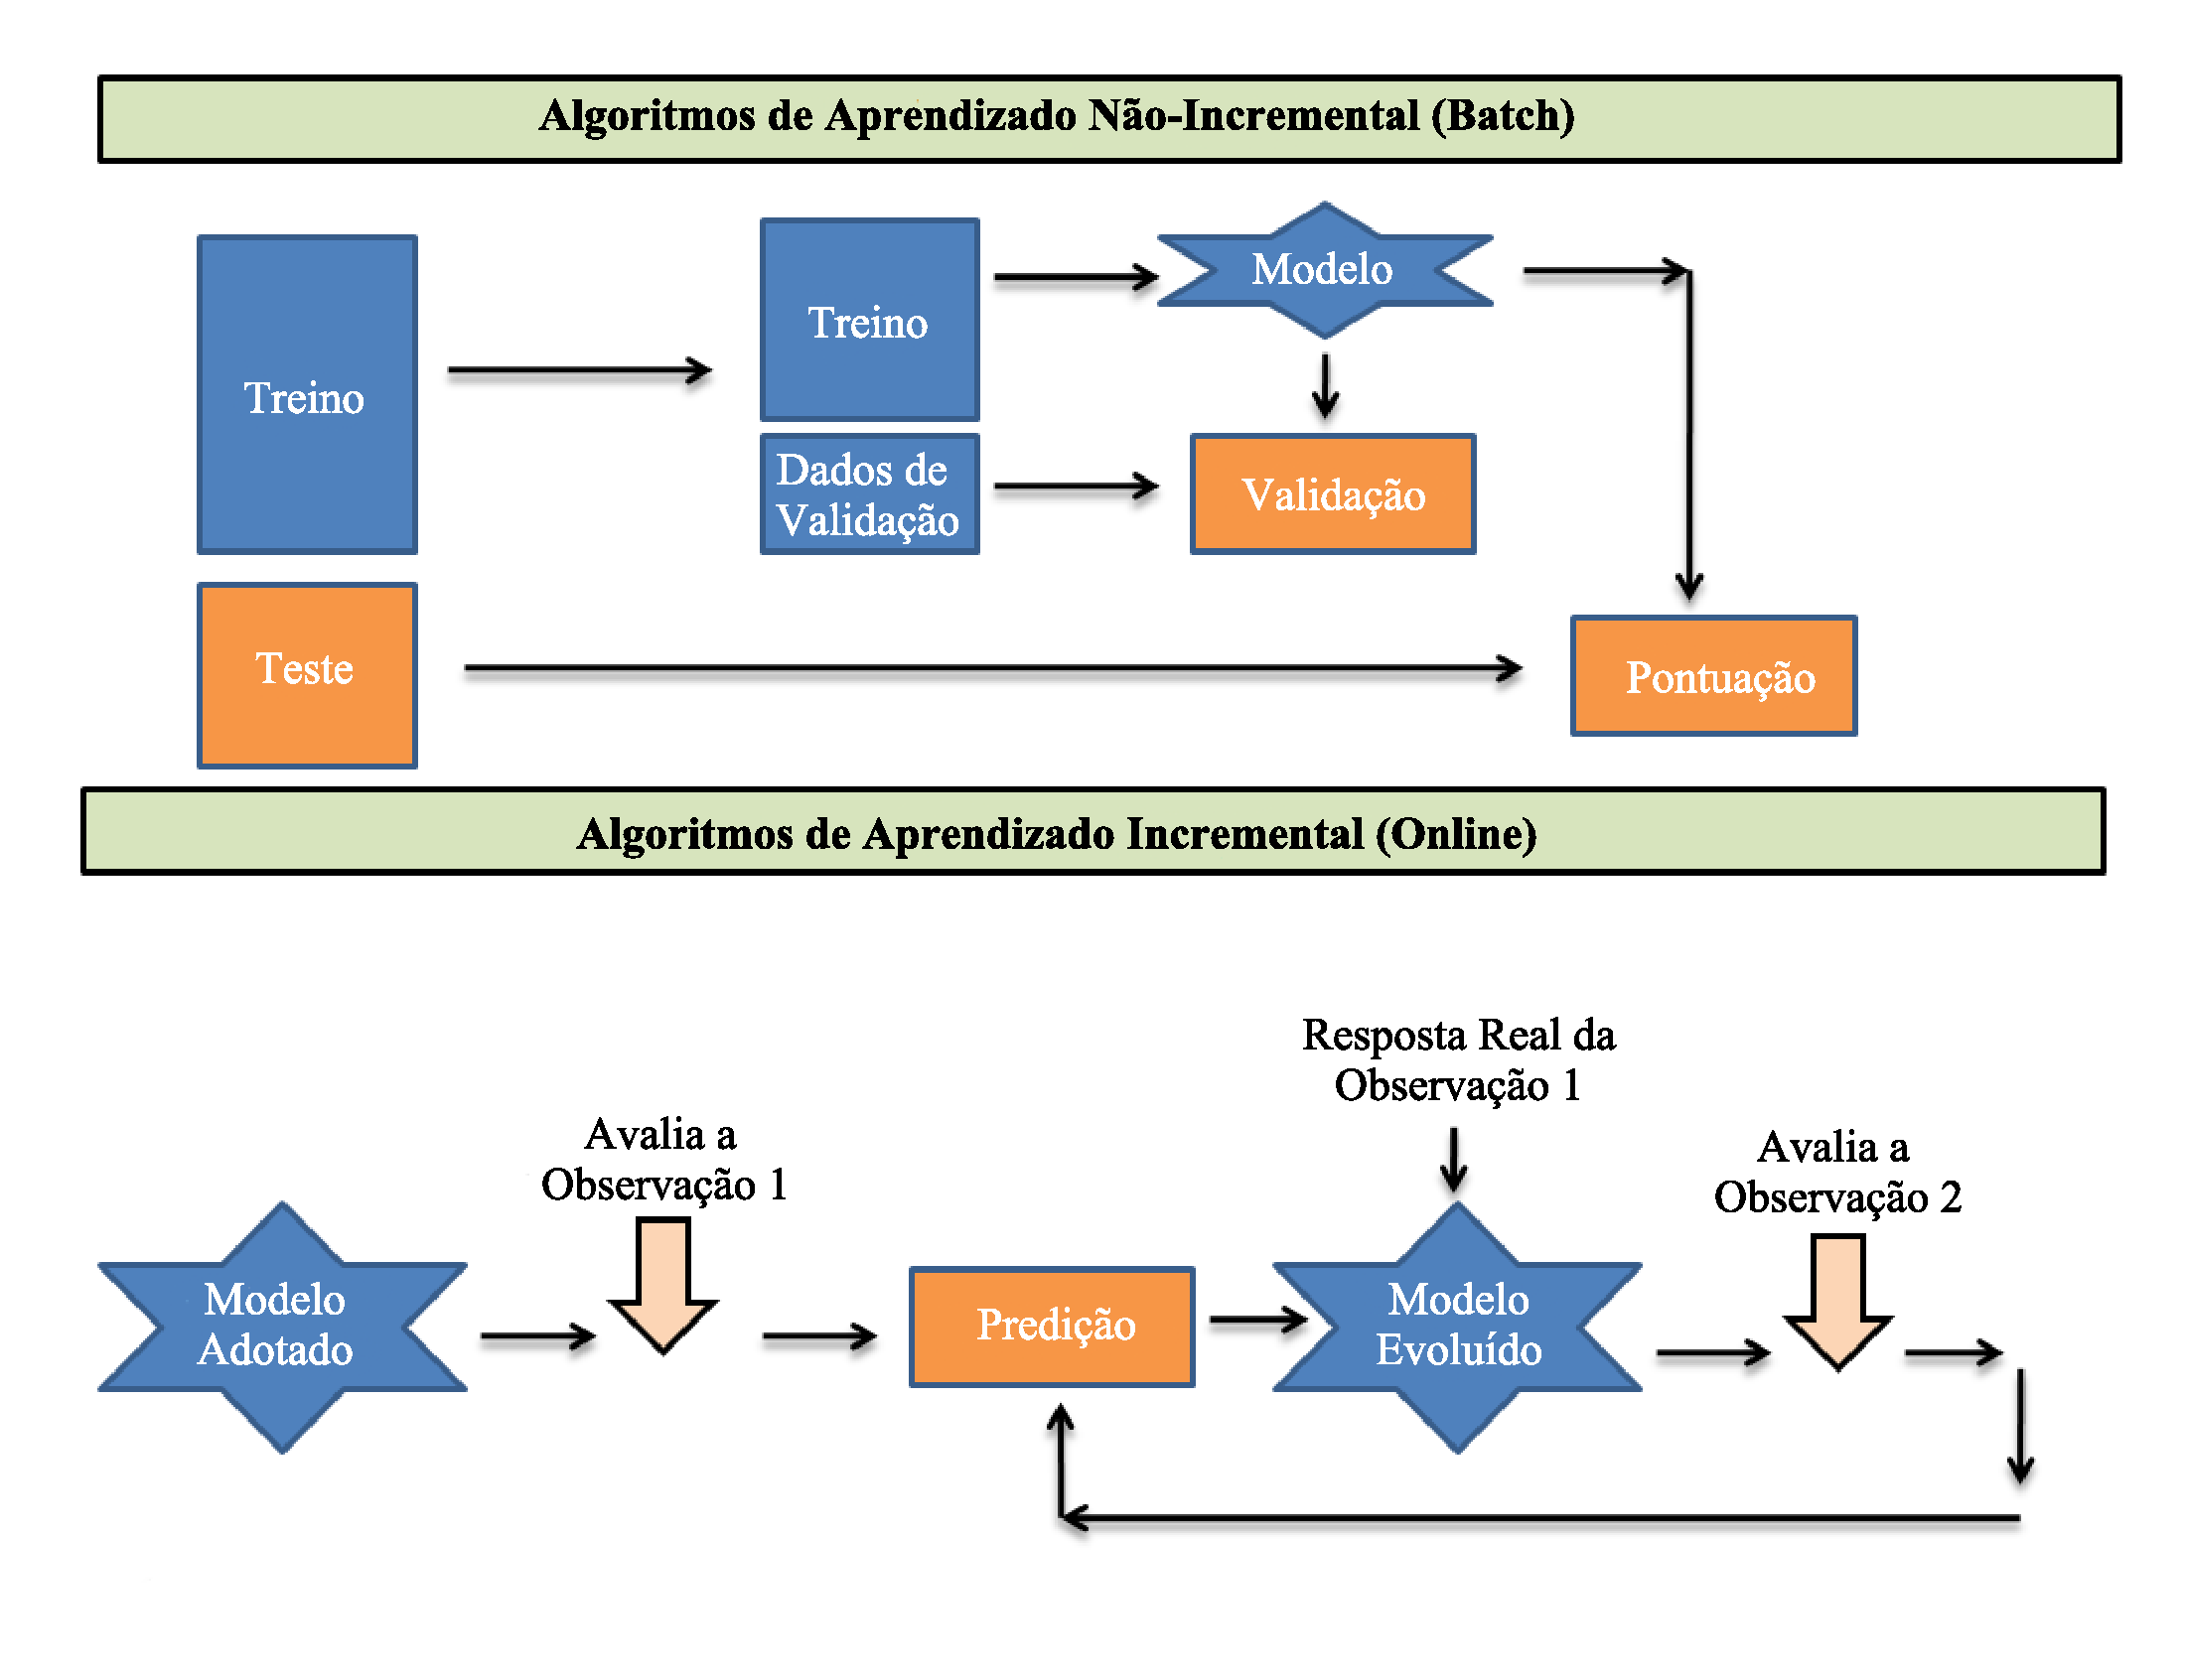
\includegraphics[width=0.9\linewidth]{aprendizado.eps}\\
	{\small Fonte: Adaptado de \citeonline{Analytics2015}.}
	\label{fig:apdz}
\end{figure}


\section{Métricas Associadas}


Para se mensurar o desempenho dos classificadores, foram considerados algumas métricas adequadas para este problema. A primeira, e mais importante, é a medida de precisão, que pode ser expressa por:

\begin{equation}
A_{cc}(R) = P(H|B) = \frac{P(HB)}{P(B)} = \frac{f_{hb}}{f_b}
\end{equation}

\noindent onde $f_{hb}$ é a quantidade de classificações corretas e $f_{b}$ é o número total de classificações. A segunda métrica utilizada é o F1-\textit{Score}, que é também uma medida de precisão, que considera também a revocação dos testes. F1-\textit{score} é obtido pela seguinte expressão:

\begin{equation}
F_1 = 2\frac{precision.recall}{precision+recall}
\end{equation}

O última medida colhida é a análise de concordância kappa (\textit{Cohen's kappa score}), que varia entre 0 e 1, os quais podem ser interpretados de acordo com a Tabela~\ref{tab:kappa}. Uma explanação mais completa destas métricas pode ser encontrado em \cite{banerjee1999beyond}.

\begin{table}[H]
	\centering
	\caption{Interpretação dos valores de Kappa}
	\label{tab:kappa}
	\begin{tabular}{ll}
		\hline
		Kappa & Interpretação \\ \hline
		\textless0 & Sem concordância \\
		0-0.19 & Concordância baixa \\
		0.20-0.39 & Concordância razoável \\
		0.40-0.59 & Concordância moderada \\
		0.60-0.79 & Concordância substancial \\
		0.80-1.00 & Concordância quase perfeita \\ \hline
	\end{tabular}
\end{table}






